\documentclass[a4paper]{exam}

% For the general maths stuff 
\usepackage{amsmath}
% For the graph drawing  
\usepackage{tikz}
% For the logic gates
\usetikzlibrary{arrows,shapes.gates.logic.US,shapes.gates.logic.IEC,calc}
\usepackage{circuitikz}
% For the pseudocode
\usepackage{algpseudocode}

% This line will remove the border around the solutions. 
\unframedsolutions
% Comment out this line to hide the solutions 
%\printanswers

\def\papertitle{LCO Summer Revision Questions}
\def\attribution{\texttt{cah@stpaulsschool.org.uk} \\ SPS Computing} 

\pagestyle{headandfoot}
\runningfooter{\papertitle}{}{\thepage}

\title{\papertitle}

\date{May 2018}

\begin{document}


\maketitle
\tableofcontents

\pagebreak
\section*{Topics} % (fold)
\label{sec:topics}

This list is not exhaustive and it appears in no particular order.

The written summer exam is (as your final exam will be) \emph{calculator} but will \textbf{not} include Python or C\#. 

In terms of the Computing text book, you should expect questions from Chapters 13--36 inclusive. For the Discrete Maths, expect questions from Chapters 1--4. 

The syllabus will be similar to the AQA AS Level (7516)\cite{syllabus-7516} and elements drawn from the OCR Further Mathematics A (H235/Y534)\cite{syllabus-h245}  

\begin{description}
\subsection*{Computing --- AQA 7516}
\item[Data representation] \hfill \\
	Number systems; 
	Bits, bytes and binary;
	Binary arithmetic and the representation of fractions;
	Bitmapped graphics;
	Digital representation of sound;
	Compression, Hashing, Encryption;
	Floating point form
\item[Computer Systems] \hfill \\
	Hardware and software;
	Role of an operating system;
	Programming language classification;
	Programming language translators;
	Logic Gates;
	Boolean algebra; 
	Adders and D-type flip flops
\item[Computer organisation and architecture] \hfill \\
	Internal computer hardware;
	The processor;
	The processor instruction set;
	Assembly language;
	Input-output devices;
	Secondary storage devices
\item[Communication and networking] \hfill \\
	Communication methods;
	Network topology;
	Client-server and peer-to-peer;
	Wireless networking, CSMA and SSID;
	Communication and privacy;
	The challenges of the digital age
\subsection*{Discrete Mathematics --- OCR Y534}
\item [Mathematical Preliminaries] \hfill \\ counting methods; $^nC_r$; pigeonhole
\item [Graphs and networks] \hfill \\ terminology, Euleran, Hamiltonian, planarity, digraphs 
\item [Algorithms] \hfill \\ measuring complexity; sorting algorithms; next-fit, first fit, first-fit descending binpacking problems.  
\item [Network algorithms] \hfill \\ least-weight paths; minimum spanning trees; Prim's, Kruskal's algorithms.
\end{description}

\begin{thebibliography}{9}
\bibitem{syllabus-7516} 
AQA Computer Science (7516) AS Level Specification 
\textit{http://www.aqa.org.uk/subjects/computer-science-and-it/as-and-a-level/computer-science-7516-7517/subject-content-as}
AQA, 2015.
 
\bibitem{syllabus-h245}
OCR Further Mathematics A 
\textit{http://www.ocr.org.uk/qualifications/as-a-level-gce/as-a-level-gce-further-mathematics-a-h235-h245-from-2017/specification-at-a-glance/\#as-level}
OCR, 2017. 
\end{thebibliography}

% section topics (end)
        

\pagebreak
\section{Binary, Hex, Numbers} % (fold)
\label{sec:binary_hex_numbers}


\begin{questions}
	\question Explain how you would turn a positive value into a two's complement number storing its negative equivalent. Use the denary values 34 and -34 and 8 bit binary values as an example.  
	\begin{solution}
		Flip the bits and add one
	\end{solution}
		
	\question The binary bit pattern \texttt{11000010} \ldots 
	\begin{parts}
		\part What is the value of this number if it is an \emph{unsigned binary integer}? \begin{solution}$194$\end{solution}
		\part What is the value of this number if it is an \emph{unsigned binary fixed point number} with 4 bits before and 4 bits after the binary point?\begin{solution}$12 \frac{1}{8}$\end{solution}
		\part What is the hex equivalent of this value? \begin{solution}$C2$\end{solution}
		\part What is the denary equivalent of this value if it represents a \emph{two's complement binary integer}? \begin{solution}$-62$\end{solution}
		\part If this number has passed parity, what style of parity is being used? \begin{solution}odd parity\end{solution}
		\part What character is being represented by this number if it represents a 7-bit ASCII code with the most significant bit being used as the parity bit? \begin{solution}$42 \rightarrow 'b'$\end{solution}
	\end{parts}

	\question Represent the following denary numbers in binary using 8 bits:
	\begin{parts}
		\part 234 \begin{solution}$11101000$\end{solution}
		\part 197 \begin{solution}$11000101$\end{solution}
		\part 57  \begin{solution}$00111001$\end{solution}
	\end{parts}

	\question How many denary values can be represented using 16 bits? \begin{solution}$2^{16} = 65536$\end{solution}

	\question What is the hexadecimal equivalent of the following denary numbers:
	\begin{parts}
		\part 289 \begin{solution}$121$\end{solution}
		\part 154 \begin{solution}$9A$\end{solution}
		\part 57005 \begin{solution}$DEAD$\end{solution} 
	\end{parts}


	\question Showing your working, multiply the binary value \texttt{1101} by \texttt{101}. 


	\question Convert the following decimal numbers to fixed point binary: 
	\begin{parts}
		\part 0.625
		\part 0.3 
		\part 0.734375
	\end{parts}

	\question Define the terms mantissa and exponent and their role in converting a binary floating point number into denary. 

	\question Convert the following decimal numbers to 8 bit two's complement, fixed point binary in which 3 bits are allocated for the fractional part: 
	\begin{parts}
		\part -1.75
		\part -6.5
		\part -14.125

	\end{parts}

	\question What is the maximum and minimum value --- in both binary and denary --- which can be stored in 8 bit signed, fixed point binary numbers in which 3 bits are allocated for the fractional part? 

	\question Convert the following floating point binary numbers which store the mantissa in 4 bits in two's complement form and the exponent in 4 bits, two's complement form, into denary. The binary point is between the most significant bit and the next ost significant bit of the mantissa. 
	\begin{parts}
		\part 01100101
		\part 10010100
		\part 01001001
		\part 01111101 
	\end{parts}
	\question What does it mean for a fixed point binary number (e.g. a mantissa in an exponent) to be normalised? 

	\question Explain the terms underflow and overflow when used with floating points numbers. 

	\question With a suitable example, explain the difference between absolute and relative errors with floating point representation. 

	


\end{questions}

% section binary_hex_numbers (end)
        

\pagebreak
\section{Information Coding}

\begin{questions}
	\question How many different ASCII codes are there? 
	\question What is the range of hex values for 
	\begin{parts}
		\part upper case letters?
		\part lower case letters?
		\part numbers?
	\end{parts}  
	\question Why has Unicode gained traction in preference to ASCII? 
	\question What would the parity bit be for the ASCII code for the letter 'A' to ensure that it passed odd parity? 
	\question Under majority voting what bits would be sent to communicate the ASCII for the number 7? 
	\question Define \emph{checkdigit} and outline either the ISBN-10, ISBN-13 or Kuhn algorithm. 
	\question In computer graphics, what is meant by the colour depth? 
	\question Relate an image's resolution to PPI. Consider the Jobsian 'Retinal Display' in your answer.
	\question Give 4 things that could be found in an image's metadata.  
	\question In a bitmapped image showing 24 bits of colour and a $1024 \times 768$ image size, how many bytes would be required? 
	\begin{solution}
	18,874,368 bits = 2.35MB
	\end{solution}
	\question For what purposes would a vector graphic format be used? Why?
	\question What attributes might you need to define to draw a circle? \begin{solution}centre (x,y), radius, fill, line, line weight, fill pattern\end{solution}
	\question Why might anti-aliasing be used on a bitmapped image after resizing?   
	\question Describe the MIDI format. 
	\question What do ADC and DAC stand for? 
	\question What aspects of sampling are required to estimate the file size? 
	\question With a bit depth of 16 bits, sampling at 44.1KHz, how many byters are required for a 60 second, single channel recording? \begin{solution}$44100 \times 60 \times 16 \div 8 = 5292000 = 5.29MB$\end{solution}    
	\question What does Nyquist's Theorem say about the relationship between sample rate and frequency? 
\end{questions}        

\pagebreak
\section{Compression, Hashing and Encryption}

\begin{questions}
\subsection{Compression}
	\question Contrast lossy and lossless forms of compression.
	\question Describe run length encoding and state whether it is lossy or lossless. 
	\question Is the storing of analogue data in digital form compression? How might such data be compressed? 
	\question Give two uses of
	\begin{parts}
		\part lossy compression 
		\part lossless compression
	\end{parts}
	\question Give three reasons why compression might be used. 
	\question Video when streamed may start being pixellated and then growing progressively smoother looking. Explain why this is the case. 
	\question What is a CODEC?

\subsection{Hashing}   

	\question What is the purpose of a hashing algorithm? 
	\question With the context of hashing, define: 
	\begin{parts}
		\part collision
		\part clustering
		\part load factor 
	\end{parts}
	\question Describe two alternative methods for dealing with collisions. 

\subsection{Encryption}
	\question Why might data be encrypted?   
	\question Define: 
	\begin{parts}
		\part key 
		\part plaintext 
		\part Caesar cipher 
		\part frequency analysis 
		\part one-time pad
		\part symmetric and asymmetric encryption  
		\part computational security 
	\end{parts} 
	\question Modulo arithmetic 
	\begin{parts}
		\part What is $21 + 15$ mod $26$?
		\part Today is Friday, what day will it be in 506 days' time? What was it 212 days ago? 
		\part If you head due East, turn through $130\deg$, what is your new bearing? 
	\end{parts}
	\question For every integer $b$ and positive integer $m$ there is exactly one integer $q$ and exactly one positive integer $r$ such that \[b = q\times m + r\], the \emph{quotient and remainder theorem}. Find $r$ and $q$ when 
	\begin{parts}
		\part $b=37, m=12$
		\part $b=76, m=60$
		\part $b=-37,m=12$
	\end{parts}

	\question Encipher a short message (< 50 characters) using a Caesar cipher. Swap with a colleague. Attempt to decipher their message. 
	\question Explain why a Vernam cipher is considered unbreakable. What conditions must be observed? 
	\question How would you set about breaking a non-trivial cipher? 
	\question How would public key crypto be used to 
	\begin{parts}
		\part encrypt 
		\part authenticate 
	\end{parts}
	messages? 
\end{questions}        

\pagebreak
\section{Software, Operating Systems, Languages}

\begin{questions}
\subsection{Software}
	\question Contrast application software with system software. 
	\question Define, with example where appropriate: 
	\begin{parts}
		\part translator;
		\part compiler;
		\part assembler;
		\part interpreter;
		\part library modules;
		\part utility program;
		\part virtual machine.
	\end{parts}

\subsection{Operating Systems}

	\question An operating systems is typified by several capabilities, define
	\begin{parts}
		\part resource management;
		\part I/O management;
		\part virtual memory;
		\part file management;
		\part UAC.
	\end{parts}
	\question Why might a user choose one operating system over another? 

\subsection{Programming Languages}
	\question Contrast machine code with assembly language. 
	\question Why might a programmer choose to code in assembly language? 
	\question Why might a programmer choose to code in a high level language? What might guide their choice of language? 
	\question With the context of high level langauges: 
	\begin{parts}
		\part imperative;
		\part functional;
		\part object-oriented;
		\part bytecode;
		\part events.
	\end{parts}


\end{questions}

\pagebreak
\section{Boolean Logic and Logic Gates}

\begin{questions}
	\question Enumerate the 6 logic gates you are expected to know. How would they be expressed in symbols? 
	\question Quote the two forms of De Morgan's Laws. 
	\question Complete the following identities:
	\begin{parts}
		\part $A\cdot0\equiv$
		\part $A+1\equiv$
		\part $A+0\equiv$
		\part $A\cdot1\equiv$
		\part $A\cdot\overline{A}\equiv$
		\part $\overline{\overline{A}}\equiv$
		\part $A\cdot A\equiv$
		\part $A\cdot (B + C)\equiv$
	\end{parts}

	\question Draw the truth table and circuit for the Boolean statement.  
			 $\overline{B} + ( \overline{\overline{A} \cdot \overline{B}} )$  
	\question Can you simplify the previous statement? 
	\question Simplify $(A+B)\cdot C \cdot \overline{C} + (A+ \overline{A}) \cdot B$ \begin{solution}$B$\end{solution} 
	\question Simplify $\overline{A+\overline{A} \cdot \overline{B}}$ \begin{solution}$\overline{A}\cdot B$\end{solution}
	\question Draw the circuit and truth table for the statement $Q = (A+B)\oplus \overline{C}$	
	\question Give Boolean statements for the following circuit diagrams:

	\begin{parts}
		\part
		
			\begin{circuitikz} \draw
				(0,2) node[nand port] (nand1) {}
				(1,0) node[not port] (not1) {}
				(4,1) node[xor port] (xor1) {}

				(nand1.in 1) node[above left=.5cm](a) {A}
				(nand1.in 2) node[below left = .5cm](b) {B}
				(nand1.out) -| (xor1.in 1)
				(not1.out) -| (xor1.in 2)
				(xor1.out) node[right=.5cm](x) {X}

				(a) -| (nand1.in 1)
				(b) -| (nand1.in 2)
				(b) node[below=1cm](c){C}
				(c) -| (not1.in)
				;
			\end{circuitikz}

		\part

			\begin{circuitikz} \draw
				(0,2) node[xor port] (myand) {}
				(4,0) node[and port] (myor) {}
				(1,1) node[not port] (mynot) {}
				(6,1) node[or port] (myxor) {}
				(myand.in 1) node[above left=.5cm](a) {A}
				(myand.in 2) node[below left = .5cm](b) {B}
				(myand.out) -| (myxor.in 1)
				(mynot.out) -| (myor.in 1)
				(myor.out) -| (myxor.in 2)
				(myxor.out) node[right=.5cm](x) {X}

				(b) -| (mynot.in)
				(a) -| (myand.in 1)
				(b) -| (myand.in 2)
				(b) node[below=1cm](c){C}
				(c) -| (myor.in 2);
			\end{circuitikz}
	\end{parts}
	\question 
	\begin{parts}	
		\part Draw a half adder.
		\part Explain --- with the aid of truth tables --- how to combine half adders together into a full adder. 
	\end{parts}
	\question Draw a logic diagram, using only NAND operations, for 
	\begin{parts}
		\part $ A + B$
		\part $ A \cdot B$
		\part $ A \oplus B$
	\end{parts}


\end{questions}

\pagebreak
\section{Internal Computer Architecture}

\begin{questions}
	\question System bus facts: 
	\begin{parts}
		\part How are the number of wires on the bus better known? What is a common value for this quantity? 
		\part What are the names for the three busses? 
		\part What direction will the data travel down these three busses? 
	\end{parts}
	\question How much address space is directly addressable by a 32-bit address bus? 
	\question Within the context of main memory, define volatile. 
	\question What does RAM stand for; explain the importance of R in this acronym. 
	\question Contrast the von Neumann and Harvard architectures.
	\question Give two reasons why I/O devices are handled by controllers rather than being connected directly to the processor. \begin{solution}Format. Speed. Monitoring new connections. \end{solution}  
	\question Explain why we would need ROM, RAM, a SSD and, potentially, a magnetic HDD within the same PC.
	\question On a games console, why might it take a minute to load a game?   
	\question Explain what is meant by the \emph{Stored Program Concept}. 
	\question Give a pro and a con for programs and data being considered as the same thing in memory. 
	\question What is meant by the clock speed? 
	\question Explain what purposes are served by the CIR, PC, MBR, MAR, SR in the fetch execute cycle. 
	\question What are the operands and the opcodes? 
	\question What are the two addressing modes? 
	\question What might cause an interrupt to be fired? 
	\question Describe the effect of an ISR on the fetch execute cycle. 
	\question Write assembly language instructions that would perform the following pseudocode, use registers $r_1$ to $r_n$ as necessary to store variables:
	\begin{algorithmic}
	\If{$A = 1$} 
		\State $B \gets 2$ 
	\Else 
		\State $A \gets A + 1$ 
	\EndIf
	\end{algorithmic}
\end{questions}

\pagebreak
\section{Input/Output}
\section{Communication}
\section{Networking}

\pagebreak
\section{Discrete Mathematics}
\begin{questions}
	\subsection{Definitions}
	\question Define: 
	\begin{parts}
		\part derangement
		\part digraph
		\part walk 
		\part trail
		\part tree
		\part hamiltonian cycle
		\part bipartite graph
		\part heuristic algorithm 
	\end{parts}
	\subsection{Classification of problems}
	\question You need to be at school by $0837$ but don't want to leave your house before $0730$. Within the context of this example, can you explain the following terms: 
	\begin{parts}
		\part existence
		\part construction
		\part enumeration
		\part optimisation 
	\end{parts} 
	\subsection{Sets and Counting}
	\question Three sets, A, B and C have 28, 28 and 22 members, $n(A\cup B \cup C) = 42$, $n(A \cap B) = 17$, $n(A \cap C) = 13$ and $n(B \cap C) = 15$. 
	\begin{parts}
		\part What is $n(A\cap B \cap C)$?
		\part If $n(\varepsilon) = 50$, what is $n(B')$?
	\end{parts}
	\question Prove that if you pick three integers at random, a pair of them will add up to an even number. \begin{solution}pigeonhole\end{solution}
	\question In a race involving 8 athletes, how many different ways can the medals for first, second and third be awarded? 
	\question In a class of 12 students, how many ways can they be split into 
	\begin{parts}
		\part 4 teams of 3;  
		\part 3 teams of 4?
	\end{parts}  

	\question How many derangements are there of the word ``NOTE''? 
	\begin{solution}
	\begin{align}
	!n &= (n-1)(!(n-1)+!(n-2)) \\
	!4 &= 9
	\end{align}
	\end{solution}
	\subsection{Graphs}
	\question A graph has nodes with degree ${2, 2, 3, 3, 4, 4}$:
	\begin{parts}
		\part Draw a possible layout for this graph, the nodes should be labelled A--F.
		\part Identify a semi-Eulerian route through your graph. 
		\part Explain whether or not your graph is simple. 		
	\end{parts}
	\question Show that there are exactly six non-isomorphic trees on six vertices. \begin{solution}Brute force \textit{https://math.stackexchange.com/questions/413792/trees-on-six-vertices}\end{solution}

	\question Using this graph: 

	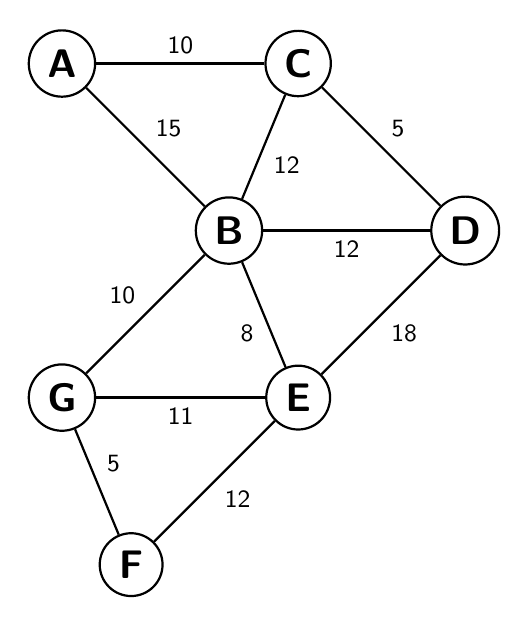
\begin{tikzpicture}[auto, node distance=3cm, every loop/.style={},
                    thick,main node/.style={circle,draw,font=\sffamily\Large\bfseries}]

		  \node[main node] (A) {A};
		  \node[main node] (B) [below right of=A] {B};
		  \node[main node] (C) [right of=A] {C};
		  \node[main node] (D) [right of=B] {D};
		  \node[main node] (E) [below left of=D] {E};
		  \node[main node] (G) [below left of=B] {G};
		  \node[main node] (F) [below left of=E] {F};

		  \path[every node/.style={font=\sffamily\small}]
		    (A) edge node  {10} (C)
		        edge node {15} (B)
		    (C) edge node {12} (B)
		        edge node {5} (D)
		    (D) edge node {12} (B)
		        edge node {18} (E)
		    (E) edge node {8} (B)
		        edge node {11} (G)
		        edge node {12} (F)
		    (G) edge node {10} (B)
		        edge node {5} (F)
		    ;
	\end{tikzpicture}

	\begin{parts}
		\part Apply Prim's algorithm and starting at `A', listing the order in which the nodes should be selected. What is the weight of your minimum spanning tree? 
		\part Apply Kruskal's algorithm, listing the order in which the nodes should be selected. What is the weight of your minimum spanning tree? 

	\end{parts}
\end{questions}

\end{document}


